\documentclass[letterpaper,10pt]{article}
% \usepackage{graphicx}
\usepackage{verbatim}
\usepackage{epsfig}

% \usepackage{}

\title{The MOOS-IvP Build System}
\author{Christian Convey (christian.convey@navy.mil)}
\date{2007-08-14}

\begin{document}

\maketitle

\begin{abstract}
This document details the design and intended use of MOOS-IvP's build system.
\end{abstract}

\tableofcontents

\parskip 7.2pt           % sets spacing between paragraphs

\section{HOWTO Build MOOS-IvP}
This section gives some basic background in using any CMake-based build system,
and then explains how to use MOOS-IvP's particular build system.

\subsection{CMake}

\subsubsection{Overview}
This section gives a brief overview of CMake, but clearer and more complete sources
of information exist:
\begin{itemize}
 \item The project's website: \verb|cmake.org|
 \item \underline{Mastering CMake}, by Ken Martin and Bill Hoffman.
 \item The CMake users email list: \verb|cmake@cmake.org|.  You can sign up
   for this at the \verb|cmake.org| website.
\end{itemize}


CMake (\verb|cmake.org|) is a cross-platform build system.  Compared to traditional 
Makefiles, CMake's control files (named \verb|CMakeLists.txt|) tend to be much shorter
and easier to read.

CMake has a number of back-ends for various operating systems and Make programs
(gmake, nmake, etc.) and IDEs (MS VisualStudio, KDevelop, Apple's XCode, etc.)
CMake-based build systems trivially support some features that can be a real
hassle to implement in hand-written Makefiles, such as calculating header file
dependencies and supporting an \verb|install| target.

The \verb|cmake| program reads in a project's \verb|CMakeLists.txt| files and produces
one or more files suitable for use in your build-system of choice (GNU Make, 
MS VisualStudio, etc.)  These generated build files will typically invoke the
\verb|cmake| program when building certain targets; therefore CMake must be installed
on any computer that will execute \verb|cmake|-produced build files.

\subsubsection{Language for Describing Makefiles}
\verb|CMakeLists.txt| files are written in an imperative language which is
documented on CMake's website.  The language lets you set variables and
supports branching, looping, and a limited form of subroutines (called
\verb|MACRO|'s).

When \verb|cmake| processes a project's \verb|CMakeLists.txt| files, the program
embodied in those files specifies the details of the build system to be created.
The \verb|CMakeLists.txt| files execute sequentially, specifying details as they
run.  Then end product is not a fully built version of your project, but rather
a set of build files (\verb|Makefile|, etc.) that when executed will build your
project.

The sequential nature of the programming language lets variables be computed,
helper programs run, conditions to be tested, etc. in order to determine what should
happen when the person building the project finally runs \verb|make| (or performs the
equivalent action in VisualStudio, XCode, etc. ).

\subsubsection{Federated Builds}
A typical CMake-based build system will contain one \verb|CMakeLists.txt| file
in each of the project's source tree's directories.  

The project's top-level \verb|CMakeLists.txt| file typically sets variables that
govern the entire project's build details, such as the directory into which 
the built libraries and / or executables should be placed after being linked, and
the directory(ies) in which the project's header files can be found.

The \verb|CMakeLists.txt| files
in the internal levels of the source tree often do nothing other than call
\verb|ADD_SUBDIRECTORY| on each of that directory's subdirectories.
(\verb|ADD_SUBDIRECTORY| is very
similar in effect to the C preprocessor's \verb|#include| directive.)
The practice of having intermediate-level directories' \verb|CMakeLists.txt|
files mostly just consist of \verb|ADD_SUBDIRECTORY| is common because
those directories often exist merely to group together 
subdirectories into units that are meaningful to the programmer.
Therefore those directories have little significance to the way the 
project code is actually built.

\subsubsection{Inherited Variables}
Consider Figure \ref{fig:cmake-file-structure}.  Using these 
\verb|CMakeLists.txt| files would look like this:
\begin{verbatim}
cmake -f CMakeLists.txt
(... some miscellaneous output from cmake ...)
Y
X
(... some miscellaneous output from cmake ...)
\end{verbatim} 

Notice how the subdirectory's file \verb|Bar/CMakeLists.txt| not 
only inherits a value of \verb|MyVar| from the parent \verb|CMakeLists.txt| 
file, but \verb|Bar/CMakeLists.txt| also affects the behavior of the
parent \verb|CMakeLists.txt| file.  (\verb|Bar/CMakeLists.txt|) modifies
the value of \verb|MyVar|, and that new value is in effect in the 
lines of the parent \verb|CMakeLists.txt| file that follow the 
\verb|ADD_SUBDIRECTORY| call.  

Contrast this to behavior to a \verb|Makefile|-based system where 
a parent directory's \verb|Makefile| calls \verb|make -f Bar/Makefile|.
In that scenario, there is no mechanims by which \verb|Bar/Makefile|'s
modifications of \verb|make| variables could propagate back to the 
parent directory's running instance of \verb|make|.

\begin{figure}
 \centering
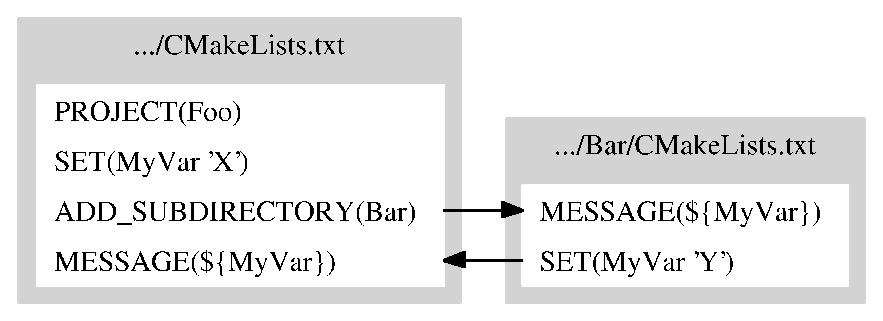
\includegraphics[width=4in]{file-structure.eps}
   \caption{ADD\_SUBDIRECTORY joines CMakeLists.txt files much like C's include}
   \label{fig:cmake-file-structure}
\end{figure}


The source tree's leaf directories typically contain the bulk of the project's 
interesting source code, with each subdirectory having the code for a single
library or executable.  The \verb|CMakeLists.txt| file in one of these leaf
directories will generally contain an \verb|ADD_LIBRARY| or \verb|ADD_EXECUTABLE|
command which leads to the compilation and linking of that one particular
program / library.

\subsubsection{Cache Files}


\subsubsection{cmake, ccmake, CMakeSetup.exe}
\subsubsection{Finding External Packages}
\subsubsection{Configuring until Stable}
\subsubsection{In-source vs. Out-of-source Builds}

\subsection{Source Tree Organization and the Two Build Systems}

\subsection{Building MOOS-Ivp}
x

\subsection{Finding Needed Files}
x

\subsubsection{FLTK}
x

\subsubsection{Python.h}
x

\subsection{Other Important CMake Variables}
x
\subsection{Builds: In-source vs. Out-of-source}

\section{Implementation of MOOS-IvP Build System }
\subsection{Each Program / Library is Optional}
\subsection{Internal Dependencies}
- If building IvP on its own, then CMake sees things like MOOSGen as
a simple library dependency, so you must build MOOS first.
- If building MOOS-IvP as a combined project, CMake knows that MOOSGen
is another build target, and will understand dependencies.

\section{Future Work}


\subsection{Debian packaging}

\subsection{RPM packaging}

\subsection{Windows builds}

\subsection{Windows packaging}

\subsection{Building Documentation}

\subsection{Building IvP's Website}

\subsection{Supporing Release Creation}


\end{document}
